%*******************************************************
% Capitulo tres
%*******************************************************

\chapter{Caso de estudio}
\label{Caso_de_estudio}

Se propone la intervención artística 'No los olvidamos' como caso de estudio para este trabajo de grado. La intervención hace parte del trabajo del colectivo artístico \textit{'Aitawa: Reconstrucción de memoria histórica con arte'}. A continuación se describe el panorama general de la obra, sus participantes, los elementos digitales o interactivos que incorpora y su metodología de construcción.

\section{Antecedentes, propósito y resultados}

Como parte de su misión, entidades gubernamentales como la 'Unidad para las víctimas' o la secretaría de Gobierno con su 'Alta consejería para las víctimas', desarrollan procesos permanentes de reparación integral para las personas que fueron afectadas directamente por el conflicto armado colombiano para que ejerzan su ciudadanía y aporten a la consolidación de la paz. Como resultado de sus acciones se han realizado talleres en el pasado que permiten la reunión de diferentes grupos de víctimas y que éstos grupos creen vínculos sociales activos. Un grupo de éstas personas se ha reunido y ha creado un colectivo para desarrollar acciones artísticas que les permitan construir lazos entre ellos, hacer catarsis de las diferentes vivencias dentro del conflicto armado, hacer visibles muchas de sus inquietudes y necesidades, desarrollar medidas de reconstrucción simbólica y de memoria y además identificar entidades que apoyen su gestión.

Una de las acciones del colectivo fue el desarrollo de una intervención artística llamada 'No los olvidamos', la cual consistió en el desarrollo de varios talleres con población inscrita en el registro único de víctimas y en la que se desarrollaban diferentes temas acerca de la reconstrucción simbólica de la memoria de algunas de las vivencias de los participantes. El proceso se orientó principalmente al flagelo de desaparición forzada y contó con el apoyo del consultorio de psicología y del Semillero en participación política, ambos del Politécnico Grancolombiano.

Durante los talleres se realizaron pequeñas piezas de origami que los participantes usaban para representar algunas de sus memorias y se realizaban guias y talleres desarrollados por los miembros del Colectivo\footnote{Los talleres y las guías no hacen parte de éste trabajo de grado y son propiedad de sus respectivos autores.}. Algunos de los talleres incluyeron acciones que permitieron utilizar la metodolgía de construcción colectiva, la cual es una metodología usada para creación artística y cuyos resultados se usaron para la aplicación de la tecnología de computación pervasiva.

Todo el proceso fue acompañado por IDARTES\footnote{Instituto Distrital de las Artes - Idartes - http://www.idartes.gov.co} en el marco de participación ciudadana de construcción del Libro al Viento 2018, para el capítulo de poblaciones el cuál será escrito por Margarita García\cite{idartesmargarita}\footnote{Margarita García Robayo visita la capital con Bogotá Contada http://www.idartes.gov.co/es/noticias/margarita-garcia-robayo-visita-la-capital-con-bogota-contada} quién participó en el último taller que el colectivo realizó.

\begin{figure}[h]\label{togafarchimate}
\centering
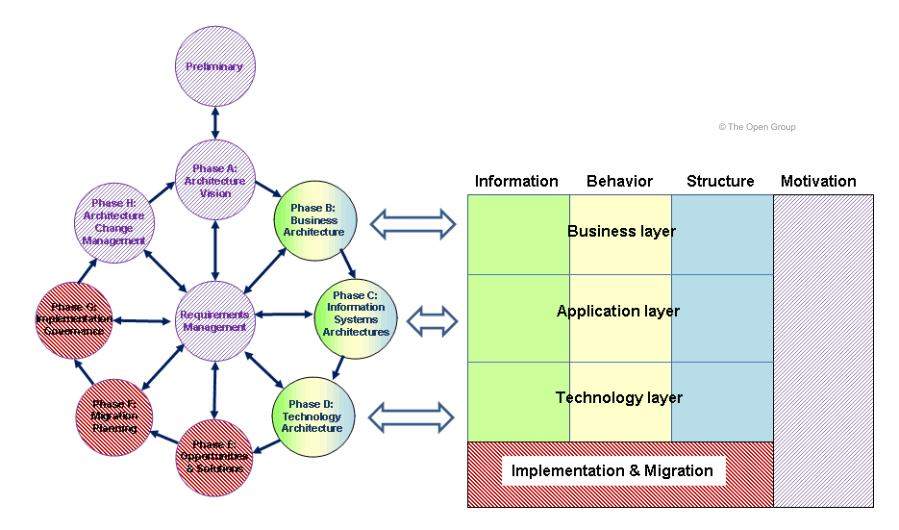
\includegraphics[scale=0.8]{togafarchimate}
\caption{Correspondencia entre Archimate y TOGAF.}
\end{figure}

\section{Talleres de construcción}

Entre las diferentes metodologías en creación de arte, el grupo decide que usará la \textit{creación colectiva}\cite{casacuberta2003creacion} y las analogías simbólicas\cite{garcia2003idea} como mecanismo para producir la obra. Numerosas obras de arte postmoderno son realizadas bajo este paradigma y en su caso las obras de arte quedan bajo la autoría de un autor principal y su grupo o bajo la autoría equilibrada de todo el grupo. Esta condición es supremamente importante en todas las decisiones que se toman frente a la aplicación de cualquier metodología de desarrollo de software. De este proceso se identifica durante el proceso realizado con los miembros del colectivo qué: 

\begin{itemize}
    \item Los requerimientos pueden cambiar ante cualquier idea que sea rápidamente aceptada por el grupo.
    \item Cada vez que los miembros del grupo desconocen uno de los elementos tecnológicos no avanzan hasta que lo comprenden del todo, incluso algunas veces no se alcanza su entendimiento.
    \item Se presenta iteraciones más numerosas en el diseño.
    \item El fin de los talleres de construcción puede ser otro al de diseñar la obra, por ejemplo describir memorias del pasado o crear piezas físicas para la obra final, por lo que se presenta confusión entre los participantes cuando se les habla de tecnología.
    \item Hay una clara distancia entre los participantes que no tienen ninguna formación técnica y el ingeniero, lo que provoca una brecha de vocabulario y comunicación.
\end{itemize}

\begin{figure}[h]\label{togafarchimate}
\centering
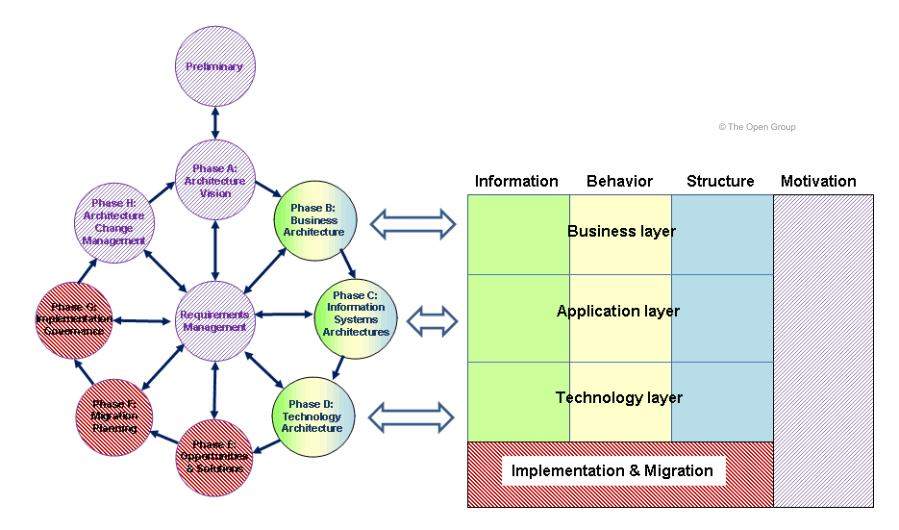
\includegraphics[scale=0.8]{togafarchimate}
\caption{Correspondencia entre Archimate y TOGAF.}
\end{figure}

Estas y otras consideraciones tiene un impacto altísimo en los modelos de proceso y las metodologías que deberían ser aplicadas en temas como este, disciplinas con las que se trabaja como ésta y en general en espacio no tradicionales de la ingeniería.  

\section{La obra}

El caso de estudio será desarrollado con la metodología de creación artística colectiva\cite{casacuberta2003creacion}. Todos los talleres desarrollados permitieron planear y construir una obra plástica digital e interactiva con la participación colectiva de los autores y los participantes de los talleres. La obra se propone como el taller final de la intervención artística y la cuál se incluye lo desarrollado en los talleres anteriores.

La presentación de la obra ocurre en el campus del Politécnico Grancolombiano en dos salones dispuestos para el evento: Uno de los salones para el desarrollo de taller y otro para la presentación de la instalación.

La obra consta de tres espacios y en dos de ellos hay elementos digitales. Tuvo un intervalo de dos horas de presentación y la coordinación, ensamble, desmontaje y convocatoria estuvo a cargo del autor de éste trabajo de grado.

\begin{figure}[h]\label{togafarchimate}
\centering
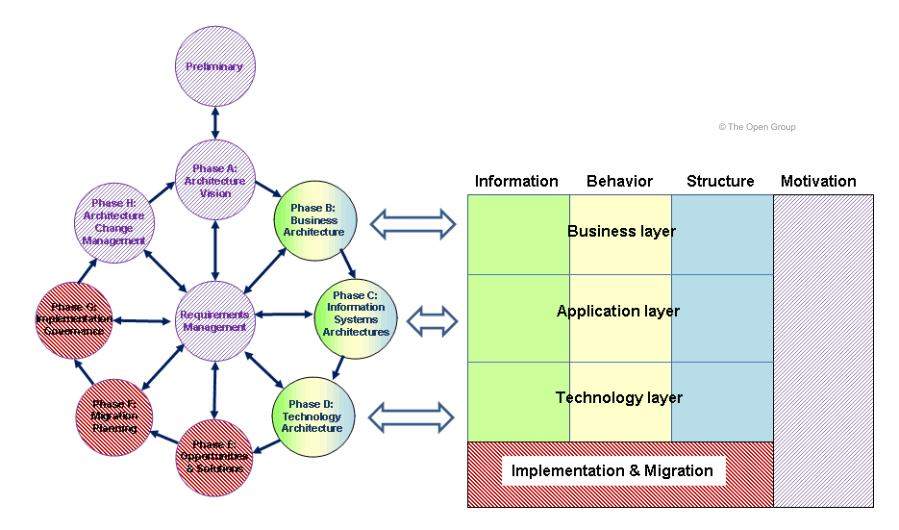
\includegraphics[scale=0.8]{togafarchimate}
\caption{Correspondencia entre Archimate y TOGAF.}
\end{figure}

\section{Los espacios}

La obra consta de tres espacios físicos: el primero de los espacios es llamado \textit{Presencia}, el segundo \textit{Ausencia} y el último \textit{Duelo}. El número tres es recurrente en la instalación y hace parte de su concepto de creación. A continuación se describen brevemente.

\begin{figure}[h]\label{togafarchimate}
\centering
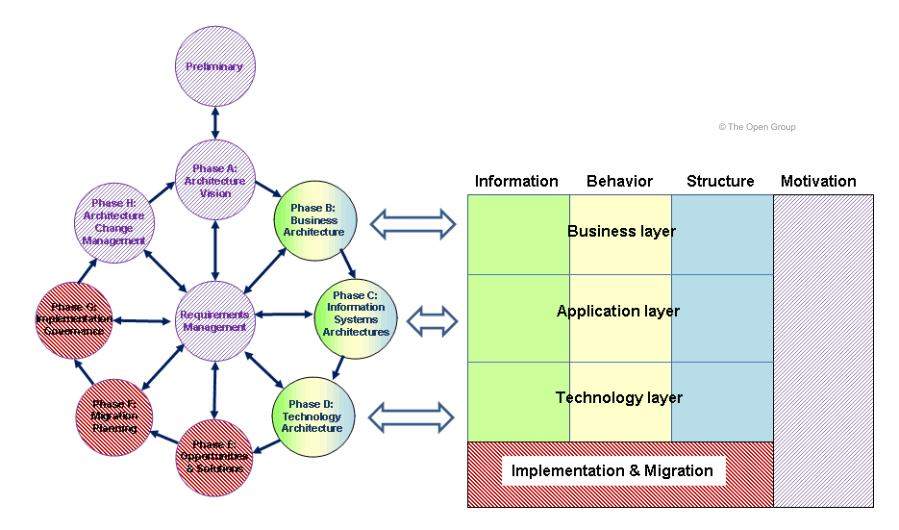
\includegraphics[scale=0.8]{togafarchimate}
\caption{Correspondencia entre Archimate y TOGAF.}
\end{figure}

\subsection{Presencia}

Es el inicio de la Instalación. El espacio consta de un mural de reconstrucción simbólica de la presencia de personas desaparecidas a partir de mariposas construidas en papel por los participantes de sesiones anteriores. En este espacio no hay ningún elemento de tecnología de forma deliverada. Tiene el objetivo de hacer contraste en la instalación y de representar la metáfora del inverso de la tecnología con la presencia humana. 

\begin{figure}[h]\label{togafarchimate}
\centering
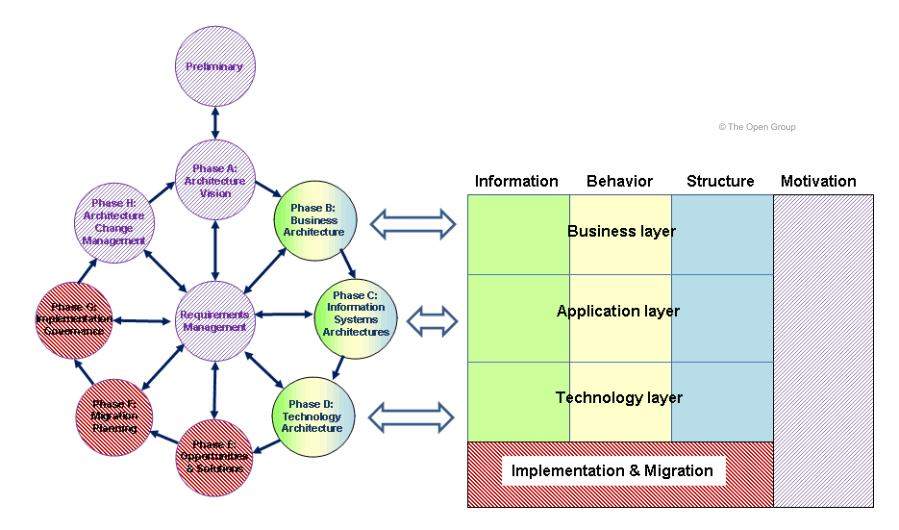
\includegraphics[scale=0.8]{togafarchimate}
\caption{Correspondencia entre Archimate y TOGAF.}
\end{figure}

\subsection{Ausencia}

Este espacio está caracterizado por una continuación del mural del primer espacio y por la presencia de objetos evocadores de memoria. Estos objetos fueron seleccionados en los talleres y componen la reconstrucción simbólica de situaciones vividas en algunos hechos violentos por los participantes. En este espacio hay tecnología de forma invisible: cuando los espectadores se acercan a los objetos se revelan imágenes en un televisor viejo dispuesto junto a los objetos. La selección de los elementos audiovisuales estuvo también a cargo de los participantes del colectivo. Este componente de tecnología es llamado el \textit{Espacio de memoria}.

\begin{figure}[h]\label{togafarchimate}
\centering
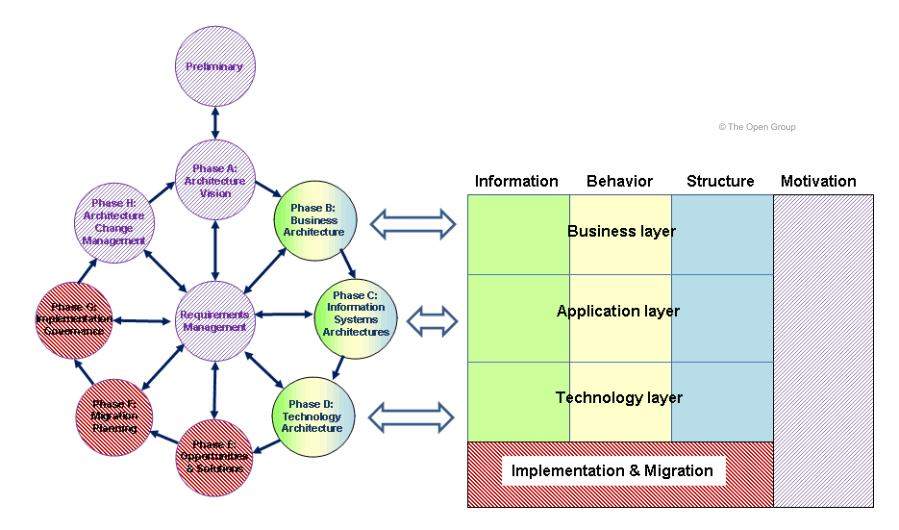
\includegraphics[scale=0.8]{togafarchimate}
\caption{Correspondencia entre Archimate y TOGAF.}
\end{figure}


\subsection{Duelo}

El último espacio representa el concepto de duelo continuado que tienen que padecer las víctimas del conflicto que sufren el fenómeno de desaparición forzada. El duelo continuado es la persistencia del estado de duelo cuando se desconoce si el desaparecido está vivo o muerto. Los familiares de desaparecidos viven en un constante estado de duelo durante el resto de su vida. Las consideraciones tecnológicas de este concepto psicológico no están contempladas como parte de este trabajo. En esta etapa hay varios elementos de tecnología que son bastante visibles y con los que se debe interactuar pero no son tradicionales: Un mural llamado \textit{El portal} se propone como componente de interacción táctil de espacio inteligente y con comunicación con el espacio anterior. Los contenidos mostrados en \textit{El portal} fueron creación del grupo y fueron desarrollados de forma colectiva.

\begin{figure}[h]\label{togafarchimate}
\centering
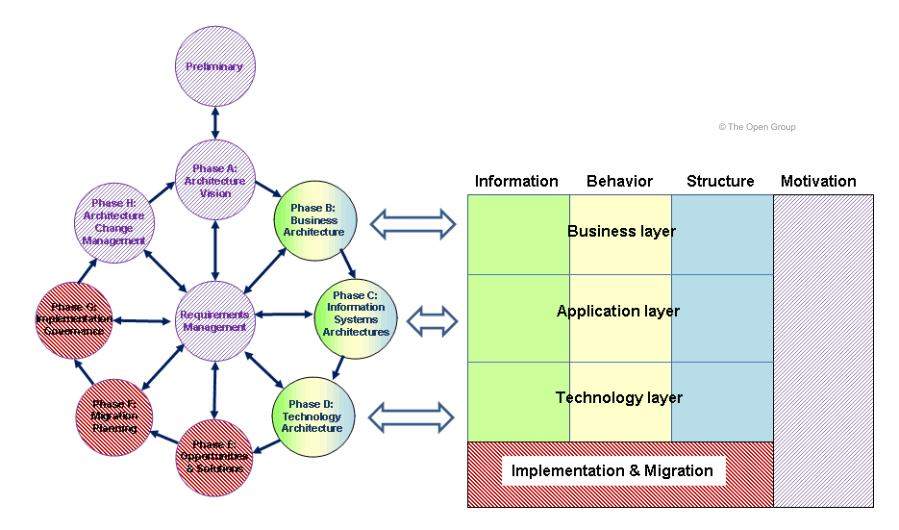
\includegraphics[scale=0.8]{togafarchimate}
\caption{Correspondencia entre Archimate y TOGAF.}
\end{figure}

\section{Componentes digitales}

Parte importante que debe ser descrita por este trabajo es el componente interactivo de la obra. El componente interactivo está representado en dos elementos ubicado en los dos últimos espacios; a saber, el primero llamado \textit{Espacio de memoria} y un segundo llamado \textit{El portal}, ambos descritos a continuación. 

\subsection{Espacio de memoria}

La reconstrucción de memoria tiene una metáfora recurrente en este espacio en donde se representan hechos vividos a través de objetos que guardan la evocación de experiencias del pasado. Cada objeto, escogido celosamente durante los talleres y el proceso de intervención, dispara una serie de recuerdos que solo la persona conoce en detalle y que hizo parte de su proceso de catarsis de las fatalidades del conflicto colombiano que tuvo que vivir.

En el espacio de memoria existe el concepto de invisibilidad de la tecnología\cite{RN13,weiser1991computer,RN23,RN14}, qué ha sido tratado por diversos autores en el contexto de computación pervasiva, en la que los humanos no se dan cuenta del computo o no se comunican de forma activa con las interfaces de usuario. Un visitante de la muestra simplemente interactuaría con los objetos y el televisor cambiaría de forma misteriosa de contenido multimedia. Es un concepto usado frecuentemente en museos y otras instalaciones interactivas, en \cite{RN31} por ejemplo, se explica  

\begin{figure}[h]\label{togafarchimate}
\centering
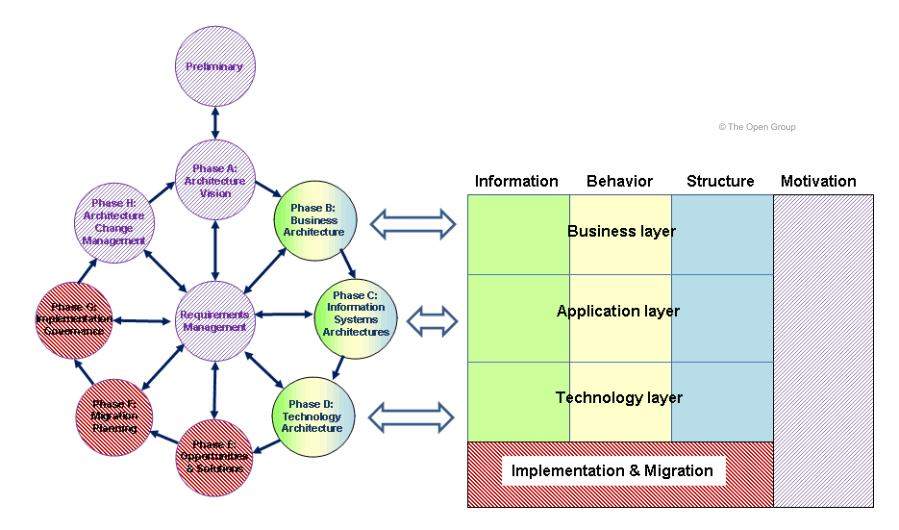
\includegraphics[scale=0.8]{togafarchimate}
\caption{Correspondencia entre Archimate y TOGAF.}
\end{figure}

\subsection{El Portal}

\begin{figure}[h]\label{togafarchimate}
\centering
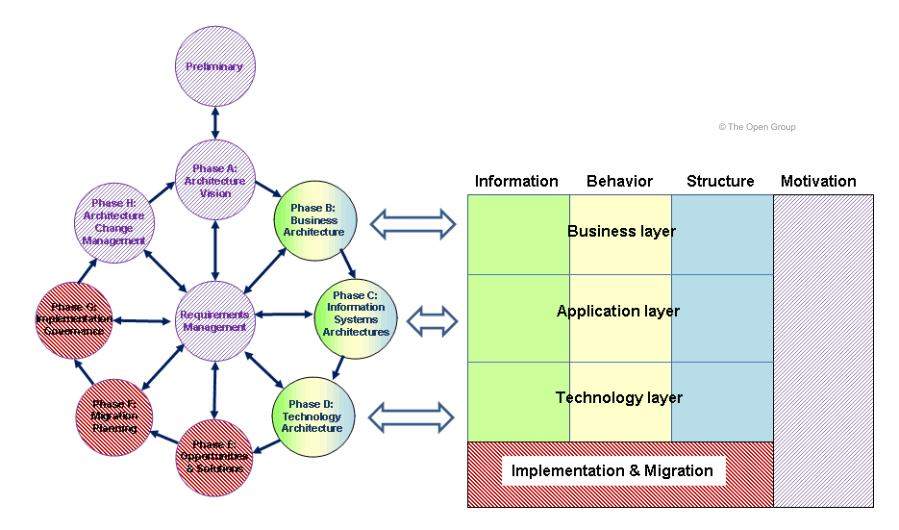
\includegraphics[scale=0.8]{togafarchimate}
\caption{Correspondencia entre Archimate y TOGAF.}
\end{figure}